    
\documentclass[11pt]{article}
\usepackage{times}
    \usepackage{fullpage}
    \usepackage{enumitem}
    \usepackage{caption}
    \usepackage{subcaption}
    \usepackage{graphicx}
    \usepackage{hyperref}
    \title{The Painter's Eye}
    \author{Caterina Mongiello - 2404262}

    \begin{document}
    \maketitle
    
    
     

\section{Status report}

\subsection{Proposal}\label{proposal}

\subsubsection{Motivation}\label{motivation}

Over the last few years, the use of AI for image generation has become increasingly popular. However, in contrast with the process that a human painter would follow, AI images are generated pixel by pixel. Moreover, painting pixel by pixel means that all the pixels receive the same amount of attention, while a human painter would focus on specific objects or parts of the image. If we want an AI agent to paint with "the eyes of a  painter" (as a human painter would), we need to change the painting process to work with brushstrokes rather than pixels, and to make the agent focus on specific parts of an image. 

\subsubsection{Aims}\label{aims}

The aim of the project is to create an AI painter agent that will paint following a process similar to the one that an actual painter would use. The agent will be composed of two main parts. The first is a neural renderer, that can generate human-like brushstrokes on a canvas. The second is a map generator. This will use the concepts of attention and saliency, as well as image segmentation, to generate a map of the most important parts of the image that will drive the painting process by making the renderer focus on these parts. 

\subsection{Progress}\label{progress}

\begin{itemize}[parsep=0pt]
  \item Frameworks chosen: the project is developed on Colab (to exploit Google's GPUs), using python and pytorch.
  \item Researched previous related projects and used them to outline the software architecture. 
  \item Neural renderer: tried different approaches and identified baseline (\href{https://github.com/jiupinjia/stylized-neural-painting}{Stylized Neural Painting}).
  \item Attention and saliency: using SalGAN to get saliency map of input image (see figure \ref{fig:salien}).
  \item Image segmentation: tried different approaches and selected the best one (Meta's Detectron) to divide the image in its components (see figure \ref{fig:segmentation}).
  \item Map generation: implemented algorithm to generate two different maps from saliency and segmentation. The first selects whole objects from segmentation if they are hit by the saliency map (object map, figure \ref{fig:final}). The second does the same, but instead of selecting the whole object, it uses the shape of the objects identified as important to mask the saliency map (blend map, figure \ref{fig:blend}).
  \item Weight distribution: implemented two approaches to distribute the focus of the painter. The first divides the image in background and foreground using the map, and gives 70\% of strokes to foreground and 30\% to background (called 'equal', figures \ref{fig:fe} and \ref{fig:be}). The second uses the map to assign a specific number of brushstrokes to each image patch. Modified the baseline neural renderer to work with the new strokes distribution (called 'individual', figures \ref{fig:fs} and \ref{fig:bs}).
  \item Experimental result: tried all the 4 approaches on the same input image to see how the results change.
  \item Generalisation: created a set of 25 images with different potential problems to see if the painter generalises well (for instance, images where the focus is not well defined).
  \item Evaluation: started looking at different quantitative and qualitative metrics to measure the performance of the painter.
  
\end{itemize}

\subsection{Problems and risks}\label{problems-and-risks}

\subsubsection{Problems}\label{problems}

Luckily, I have not encountered any major issue with the project this far. However, there were some minor problems. 
\begin{itemize}[parsep=0pt]
    \item Colaboratory quickly started complaining about GPU usage, solved by subscribing to Colab pro.
    \item Dealing with all the checkpoint files for the various networks was challenging, since my computer has limited memory. Right now the solution was to store them on Google Drive, and I will switch to GitHub over the Christmas break.
    \item Changing the original painting algorithm was difficult because of all the operations on tensors, and it required a lot of step-by-step debugging. This was made harder by the way in which Colab handles variables: sometimes, fixing the code would not fix the error. The solution was to restart the runtime every time I modified one of the files imported in the notebook, to make sure changes were mirrored in the notebook variables.
\end{itemize}

\subsubsection{Risks}\label{risks}

\begin{itemize}[parsep=0pt]
    \item Colab's GPUs easily run out of memory when input images are too big. \textbf{Mitigation:} will create a preprocessing function to resize the images to a standard size.
    \item If the image has a lot of white and the starting color of the canvas is white, it leaves the white spaces without painting on top of them, which is not good aesthetically (the same happens with black). \textbf{Mitigation:} will create a function to decide on the starting color based on the color of the image (if the image is mainly white start with black canvas and vice-versa).
    \item It is quite challenging to find appropriate quantitative metrics to measure performance, as the ones identified from the literature measure the pixel difference with the original image, which is bound to be very different in terms of texture and style. \textbf{Mitigation:} ???
\end{itemize}

\subsection{Plan}\label{plan}
\begin{itemize}[parsep=0pt]
    \item Week 1-3: Modify and improve code, plan evaluation. Finish writing first part of the draft.
        \begin{itemize}
            \item \textbf{Deliverable:} polished software ready for evaluation.
        \end{itemize}
    \item Week 4-6: Run evaluation and collect data. Write the second part of the draft.
        \begin{itemize}
            \item \textbf{Deliverable:} evaluation results and dissertation draft.
        \end{itemize}
    \item Week 7-8: Write proper dissertation and prepare video presentation
    \item Week 9-10: Proofreading (will not be able to work much on the project due to a theatre placement)
    \item Week 11: Check last details and submit.
        \begin{itemize}
            \item \textbf{Deliverable:}  dissertation and presentation.
        \end{itemize}
\end{itemize}


\begin{figure}[h]
     \centering
     \begin{subfigure}[b]{0.25\textwidth}
         \centering
         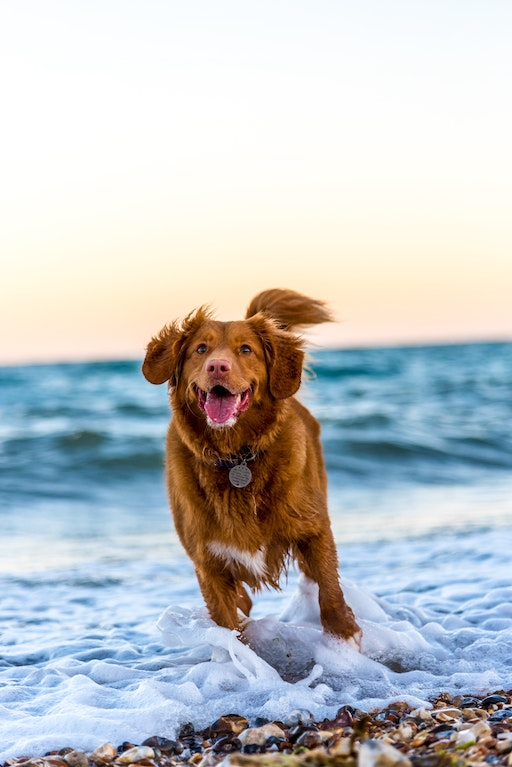
\includegraphics[width=\textwidth]{animal-centre2.jpg}
         \caption{Input image}
         \label{fig:input}
     \end{subfigure}
     \begin{subfigure}[b]{0.25\textwidth}
         \centering
         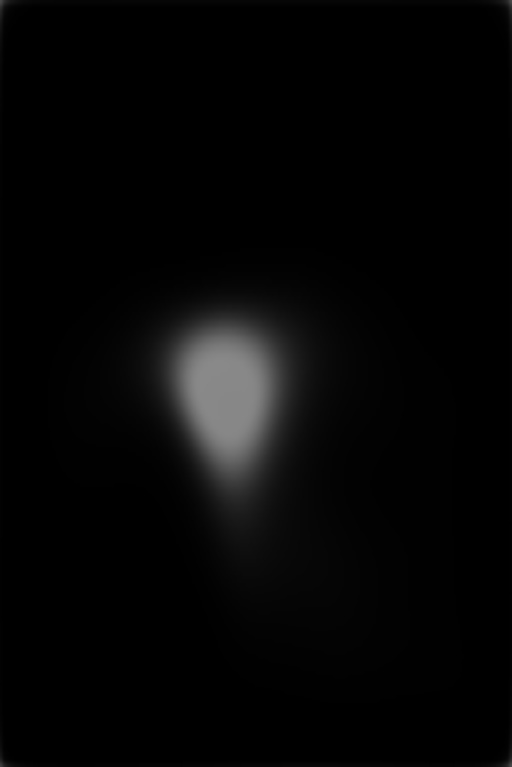
\includegraphics[width=\textwidth]{animal-centre.jpg}
         \caption{SalGAN's Saliency map}
         \label{fig:salien}
     \end{subfigure}
\end{figure}


\begin{figure}[h]
     \centering
     \begin{subfigure}[b]{0.25\textwidth}
         \centering
         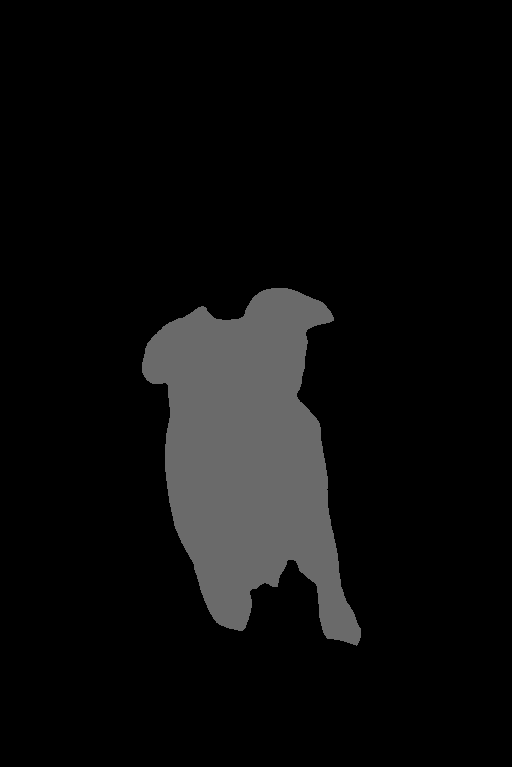
\includegraphics[width=\textwidth]{dog.png}
         \caption{dog}
         \label{fig:y equals x}
     \end{subfigure}
     \begin{subfigure}[b]{0.25\textwidth}
         \centering
         
\includegraphics[width=\textwidth]{sea.png}
         \caption{sea}
         \label{fig:three sin x}
     \end{subfigure}
     \begin{subfigure}[b]{0.25\textwidth}
         \centering
         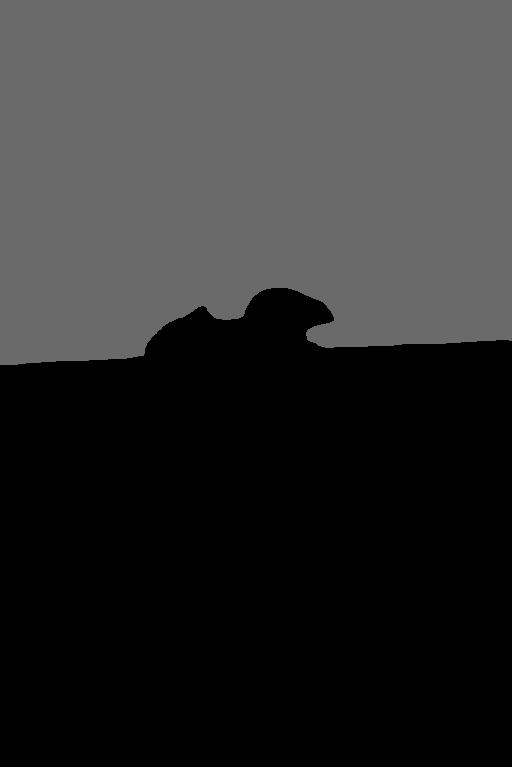
\includegraphics[width=\textwidth]{sky-other-merged.png}
         \caption{sky}
         \label{fig:five over x}
     \end{subfigure}
        \caption{Figure segmentation with detectron}
        \label{fig:segmentation}
\end{figure}

\begin{figure}[h]
     \centering
     \begin{subfigure}[b]{0.25\textwidth}
         \centering
         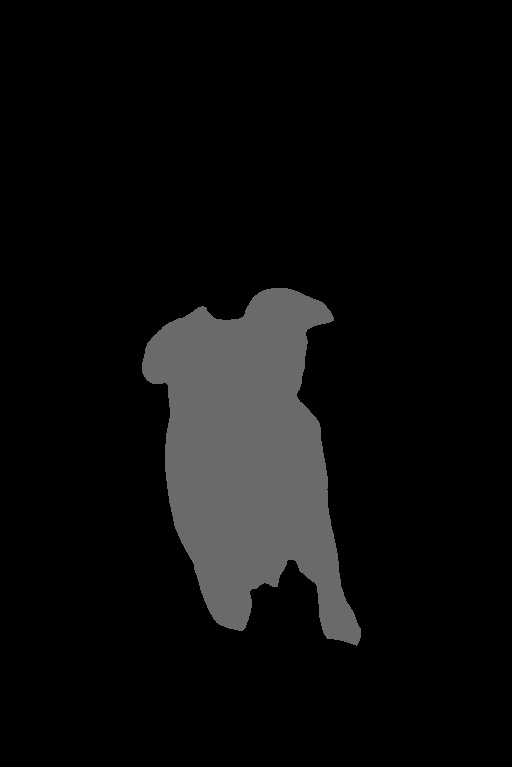
\includegraphics[width=\textwidth]{final-2.jpg}
         \caption{object map}
         \label{fig:final}
     \end{subfigure}
     \begin{subfigure}[b]{0.25\textwidth}
         \centering
         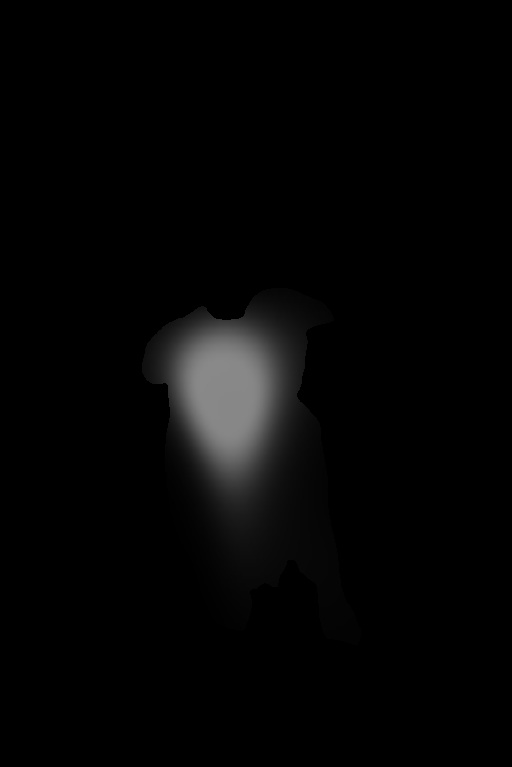
\includegraphics[width=\textwidth]{finalblend-2.jpg}
         \caption{blend map}
         \label{fig:blend}
     \end{subfigure}
     \caption{The final maps to drive the painting process}
    \label{fig:maps}
\end{figure}

\begin{figure}[ht]
     \centering
     \begin{subfigure}[b]{0.24\textwidth}
         \centering
         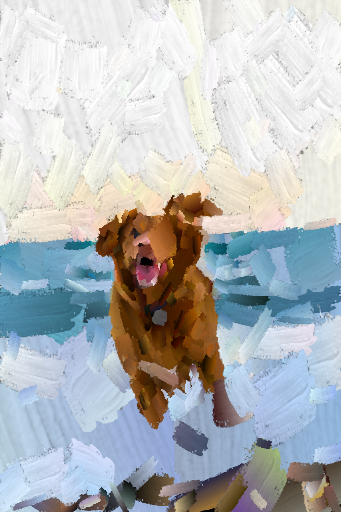
\includegraphics[width=\textwidth]{final-equal.png}
         \caption{object map and equal weights}
         \label{fig:fe}
     \end{subfigure}
     \hfill
     \begin{subfigure}[b]{0.24\textwidth}
         \centering
         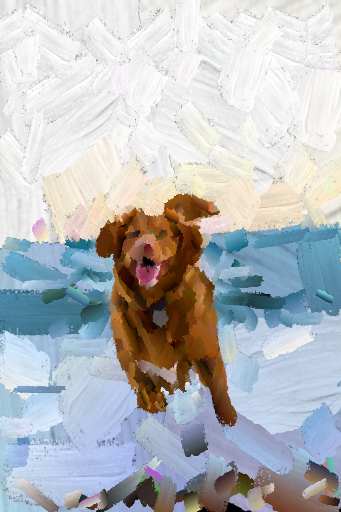
\includegraphics[width=\textwidth]{blend-equal.png}
         \caption{blend map and equal weights}
         \label{fig:be}
     \end{subfigure}
    \hfill
     \begin{subfigure}[b]{0.24\textwidth}
         \centering
         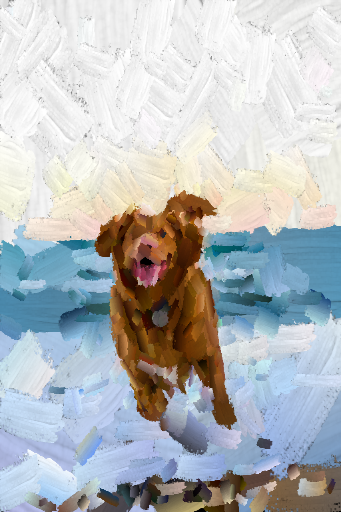
\includegraphics[width=\textwidth]{final-singular.png}
         \caption{object map and individual weights}
         \label{fig:fs}
     \end{subfigure}
     \hfill
     \begin{subfigure}[b]{0.24\textwidth}
         \centering
         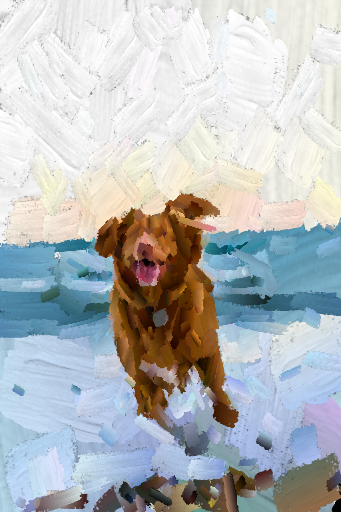
\includegraphics[width=\textwidth]{blend-singular.png}
         \caption{blend map and individual weights}
         \label{fig:bs}
     \end{subfigure}
      \caption{The final results on the input with the 4 algorithms}
    \label{fig:results}
     
\end{figure}

\end{document}
